\begin{lstlisting}
习题2:
2,(1)(2)
3,(3)(4)(7)(8)(9)
\end{lstlisting}
\begin{figure}[H]
\centering
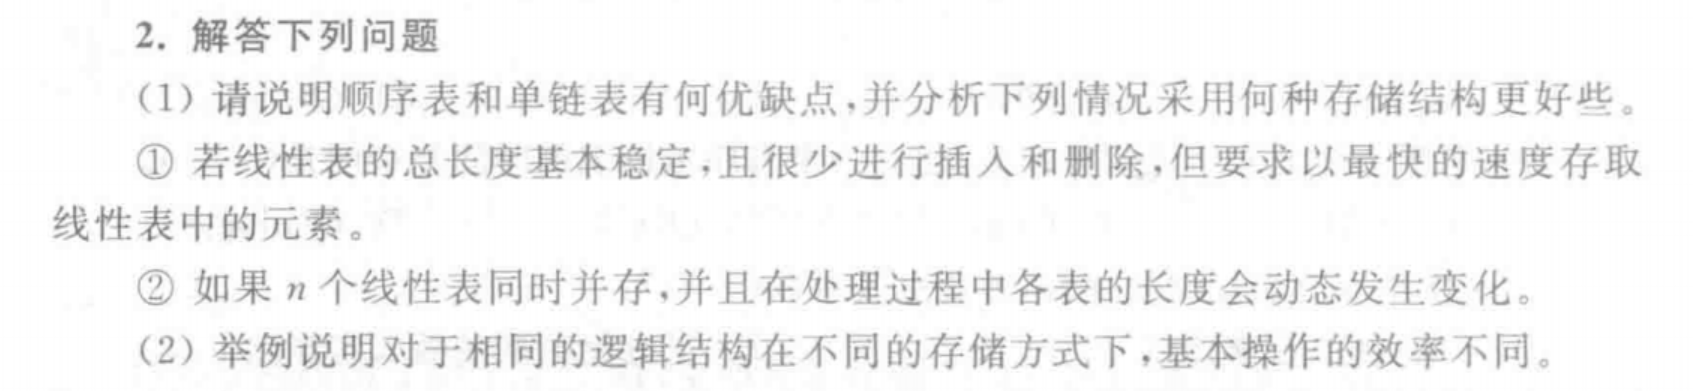
\includegraphics[width=\textwidth]{hw2-2025040120.png}
% \caption{}
\label{}
\end{figure}

\begin{table}[h]
	\centering
	\begin{tabular}{|c|c|c|}
		\hline
		\textbf{存储结构} & \textbf{优点} & \textbf{缺点} \\
		\hline
		\textbf{顺序表}(数组) & 1. \textbf{支持随机访问},时间复杂度为 O(1)。  <br>2. 结构简单,存储密度高(即没有额外指针存储开销)。 & 1. \textbf{插入和删除操作效率低},平均时间复杂度为 O (n)(需要移动元素)。  <br>2. \textbf{长度固定或动态扩容成本高},如果事先分配的空间过小或过大,都会影响效率。 \\
		\hline
		\textbf{单链表} & 1. \textbf{插入和删除操作效率高},时间复杂度为 O(1)(在已知插入/删除位置的情况下)。  <br>2. \textbf{支持动态存储},可根据需要灵活调整长度。 & 1. \textbf{不支持随机访问},查找元素需要遍历,时间复杂度为 O(n)。  <br>2. \textbf{额外存储开销大},每个结点需要额外存储一个指针。 \\
		\hline
	\end{tabular}
\end{table}
(1)
1️⃣顺序表
2️⃣单链表

(2)
比如查找操作,对于长度为 $n$ 的数据,要查找第 $k$ 个位置的数据,顺序表的时间复杂度为 $O(1)$,而单链表的时间复杂度为 $O(n)$. 代码如下:

\begin{lstlisting}[language=C++]
// 顺序表(数组)查找第 k 个元素(O(1))
int find_k(int arr[], int k) {
    return arr[k];  // 直接索引访问
}

// 单链表查找第 k 个元素(O(n))
Node* find_k(Node* head, int k) {
    Node* p = head;
    for (int i = 0; i < k; i++) {
        p = p->next;
    }
    return p;  // 需要逐个遍历
}
\end{lstlisting}
\begin{figure}[H]
\centering
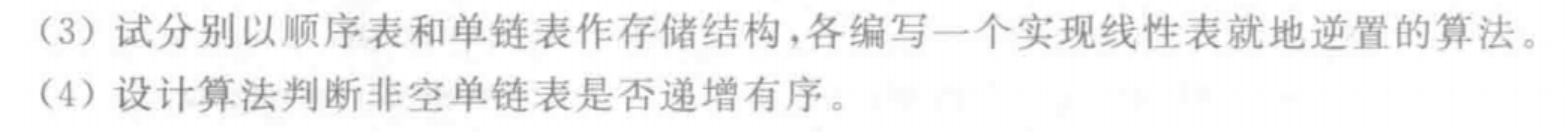
\includegraphics[width=\textwidth]{1-hw2-2025040120.png}
% \caption{}
\label{}
\end{figure}

(3)
顺序表就地逆置:

\begin{lstlisting}
input: 顺序表A, 长度n
output: 逆置后的顺序表

left=0
right=n-1

while left<right do
    p = A[left]
    A[left] = A[right]
    A[right] = p
    left++
    right--

return A
\end{lstlisting}
单链表就地逆置:

\begin{lstlisting}
input: 单链表头指针first
output: 逆置后的新的头指针

prev = NULL
p = first

while p != NULL do
    q = p->next
    p->next = prev
    prev = p
    p = q

return prev
\end{lstlisting}
(4)
判断非空链表是否非空有序

\begin{lstlisting}
input: 单链表头指针first
output: true/false

p = first->next

while p->next != NULL do 
    q = p->next
    if p.value > q.value
        return false
    p = q

return true
\end{lstlisting}
\begin{figure}[H]
\centering
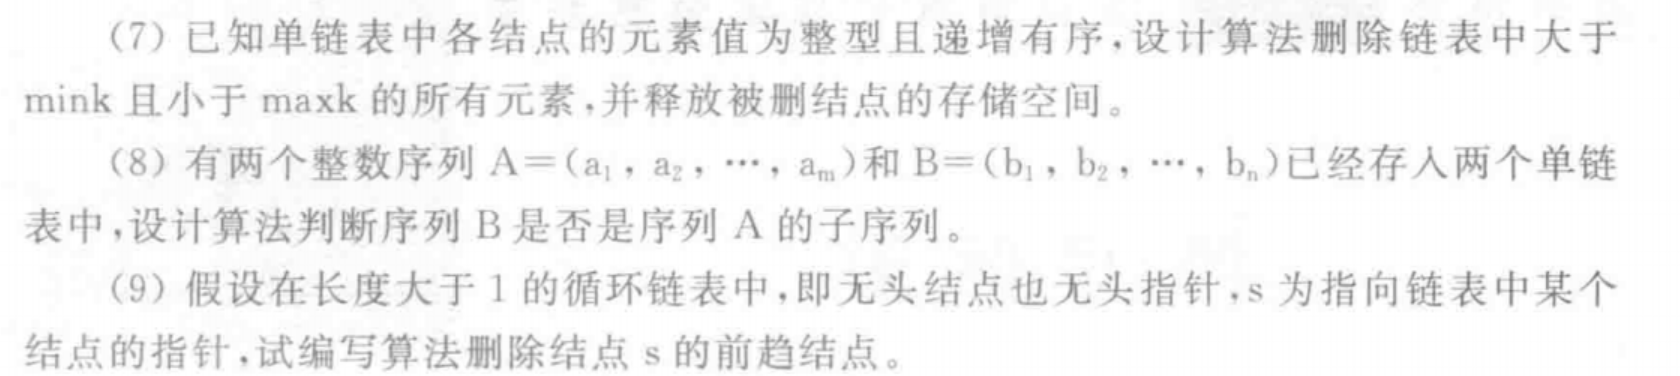
\includegraphics[width=\textwidth]{2-hw2-2025040120.png}
% \caption{}
\label{}
\end{figure}

(7)
先找出 \lstinline{mink} 和 \lstinline{maxk},然后再删去大于 \lstinline{mink} 且小于 \lstinline{maxk} 的所有元素,并释放被删节点的储存空间.

\begin{lstlisting}
input: 单链表头指针first
output: 新的单链表

p = first
mink = p->next->value

q = p
while q->next != NULL do
    q = q->next

maxk = q->value

while p->next->value != maxk do
    q = p->next
    if q->value > mink && q->value < maxk
        p->next = q->next
        release(q)

\end{lstlisting}
(8)

\begin{lstlisting}
input: 指向序列 A 的单链表头指针 a, 指向序列 B 的单链表头指针 b
output: True/False 

currA = a
currB = b

while currA ≠ NULL do
    if currA.value = currB.value then
        currB ← currB.next  // B 继续匹配下一个元素
        if currB = NULL then
            return True  // B 完全匹配成功

    currA ← currA.next  // A 继续向后遍历

return False  // A 遍历完,B 仍未匹配完
\end{lstlisting}
(9)

\begin{lstlisting}
Input: s(循环单链表中的一个指针)
Output: 删除 s 的前驱结点后,链表的修改

p = s
while p->next->next != s do
    p = p->next

q = p->next
release(q)
p->next = s
\end{lstlisting}